\chapter{Online Learning Algorithms}
\label{ch:online-learning}\index{online-learning}

\section{Introduction}

\begin{figure}
  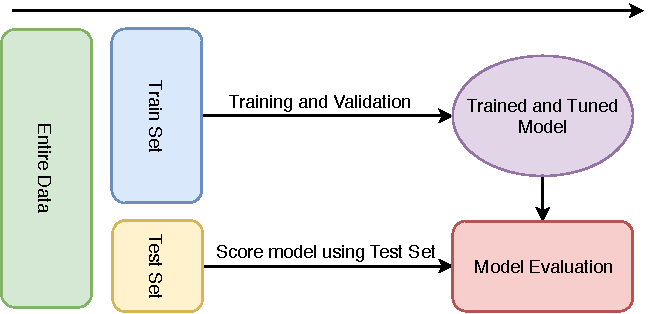
\includegraphics{online_learning/traditional.pdf}
  \caption{The traditional batch train-test machine learning approach workflow.}
  \label{fig:traditional_ml}
\end{figure}

In the traditional machine learning approach depicted in Figure~\ref{fig:traditional_ml}, we usually have some historical data to train an algorithm on for predicting some future events \citep{oza_online_2005}. However, since most data environments are dynamic and will change, the trained model eventually becomes outdated. To tackle this, we usually automate model re-training based on a timeframe (i.e.\ weekly or daily basis). Although this helps with keeping the model up-to-date, this is still not enough. Even if we consider model re-training on a daily basis, the model would still be at least one day late. 

Furthermore, as \citet{pagels_what_2018} argued, no matter how good a specific model is, it would always be an imperfect representation of the problem. Moreover, to have the best prediction for today, we cannot rely on a model with knowledge about yesterday only. Enter online learning algorithms, a family of techniques that are modelled to consume as much data available (one sample at a time), as fast as possible, while continuously learning and adapting different learning parameters. In the following sections, we will dive deeper into the subject of online learning, and its particular usage.

\begin{figure}
  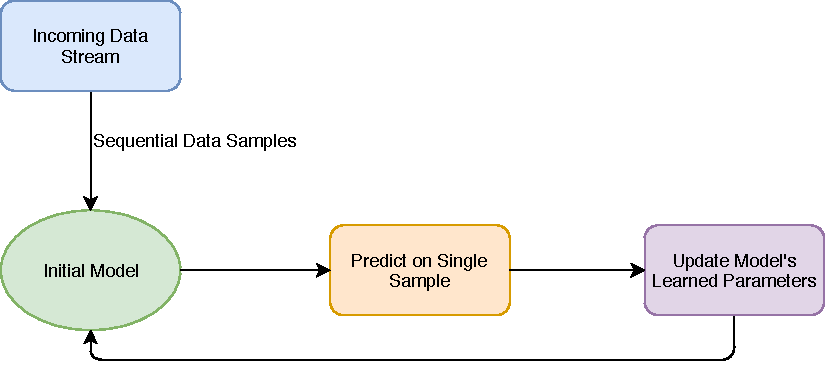
\includegraphics{online_learning/online.pdf}
  \caption{Basic workflow architecture of online learning.}
  \label{fig:online_ml}
\end{figure}

\section{Why use Online Learning?}

While being highly adaptable to dynamic underlying data structures since they make no statistical assumptions on the distribution of the data \citep{hoi_libol:_2014}, online learning techniques are also highly data efficient. Since online learning algorithms are only updated using the most recent data samples in the stream (as illustrated in figure~\ref{fig:online_ml}), such data samples are no longer stored or needed once the algorithm has passed over them, maintaining a much smaller data storage \citep{oza_online_2005}. Such algorithms are also very fast since only a single pass on a smaller data set is made, in contrast to the standard approach where the optimisation function needs multiple iterations over the entire dataset. Thus, as argued by \citet{hoi_online_2018}, online learning algorithms scale much better than the traditional approach.

As aforementioned, in offline machine learning, we load an entire dataset in memory, process it, then train a specific model, and then deploy the model into production. However, as more and more data is being generated, especially with the bright spotlight on Big Data, this methodology is proving to be more and more tedious. Some data sets are too large to fit into memory, even with distributed computing measures in place. Thus, online learning can drastically help in this scenario due to its small data storage property, especially when considered as online distributed computing and out-of-core computation \citep{zhang_projection-free_2017}, which is a huge plus.

To further extract the important usability of online learning, let us, as an analogy, consider the case of an online news portal where news articles are custom and shown to the users based on which categories that respective user usually tends to click. Pretending that a terrible disaster is happening or has happened on one specific day, and the government issues a 24-hour emergency evacuation; therefore, the majority of the user-base would start clicking on this news more and more. With the traditional batch approach, even with a re-training time of 24 hours, the system would fail to push this article to users who typically do not click on domestic affairs articles (i.e.\ users only interested in sports or entertainment). As a result, the same data content structure will be assumed by the algorithm even though there was a drastic change of events. 

In addition to this, given the same batch algorithm, after re-training in the following day, it would now start to suggest this article to a high percentage of the user-base, which by this time, such news might no longer be relevant or applicable.

Another small application resides in the online advertising domain. With different events and occasions happening every day, especially unscheduled or unforeseeable events which go viral, ads must stay relevant all the time to ensure the highest click-rate probability, and thus, must always synchronise to the affairs of the physical world. Ads must be intelligent enough to be aware of the hidden data distribution to adapt to data morphism.

In both examples, a traditional static model will fail due to being too slow to react to the dynamic underlying relationships present in the data. This problem is more formally known as concept drift \citep{schlimmer_incremental_1986}. The following section will further explain the notion of Concept Drift.

\section{Concept Drift} \index{online-learning!concept drift}

Concept Drift occurs when the hidden context of the data changes. For instance, weather predictions are highly dependant on the season (the context), and as the seasons change so does the weather \citep{widmer_learning_1996}. As highlighted by \citet{krawczyk_online_2018, Gama2014ASO}, based on the distribution drift speed and severity, concept drift can be of four types as depicted in Figure~\ref{fig:cd}:

\begin{figure}
  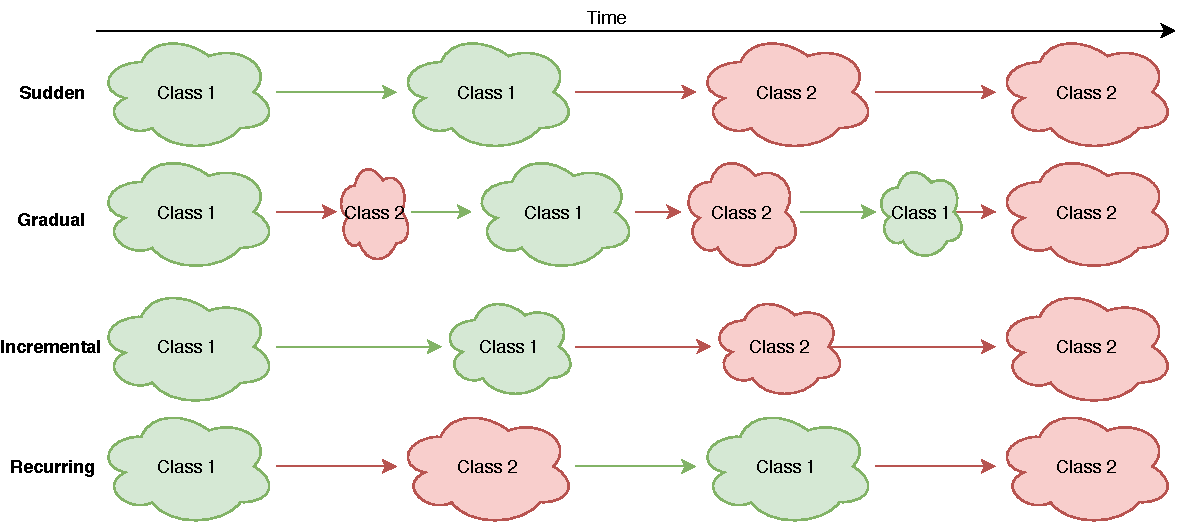
\includegraphics{online_learning/cd.pdf}
  \caption{The four types of Concept Drift.}
  \label{fig:cd}
\end{figure}

\begin{enumerate}
\item \textbf{Sudden:}\index{online-learning!sudden drift}
\textit{The data distribution is immediately changed to a different class.}
\item \textbf{Gradual:}\index{online-learning!gradual drift}
\textit{The data distribution gradually transitions by having varying proportions of the different classes mixing together over time, until it completely changes to the new class.}
\item \textbf{Incremental:}\index{online-learning!incremental drift}
\textit{The data distribution slowly morphs from one class to another.}
\item \textbf{Recurring:}\index{online-learning!recurring drift}
\textit{The data distribution periodically transitions between previous classes.}
\end{enumerate}

\subsection{Dealing with Concept Drift}

Thus, to combat this, as the concept drifts, so must the model's transition function that maps the inputs to the outputs. Due to the constant model updates performed through online learning (sample by sample), the transition function would be dynamic and adapts to the changing distribution \citep{Gama2014ASO, hoi_online_2018, Lane:1998:AOL:3000292.3000339}. In addition to this, another approach is to have a sliding window that shifts with the data stream. The purpose of this window, as discussed by \citet{wozniak_hybrid_2011}, is to keep a set of instances that offer the best representation of the present data distribution. As newer data samples arrive in the stream, the window slides towards more recent instances, resulting in the exclusion of the oldest samples from the window. Online learning achieves this window technique through the 'forgetting rate' which sets how fast older data is discarded to make room for newer instances. 

\subsection{Forgetting Rate}\index{online-learning!forgetting rate}

Even though the design for most online learning algorithms is for fast execution speeds and thus adapted from less complex algorithms, implementation challenges are also present. As argued by \citet{gepperth_incremental_2016}, this leads us to one of the most significant problems in online learning, Catastrophic Interference. The latter happens when the model abruptly forgets knowledge learnt for previous data. Most online learning algorithms have a forgetting rate parameter. This parameter allows the user to decide the speed at which the learning algorithm forgets old data; thus, how much data to retain. Moreover, the correct calibration of this rate is essential and challenging to perfect since a high value would result in catastrophic interference, while a lower value would result in the algorithm not adapting to the incoming samples in the stream. In addition to this, good initialisations are critical in this approach to steer away from slow convergence.

\section{Conclusion}

In this chapter, we introduced and discussed the sub-field of online learning algorithms concerning machine learning. Online learning is a highly useful tool that allows us to take machine learning to a whole other level by solving problems that otherwise would seem to be out of our technical ability. With the exponential importance for Big Data analytics, online learning arms us with the capabilities to process high-velocity data while also being fast to adapt to frequent changes in the data due to the ever-increasing data velocity.